\documentclass{article}
\usepackage[utf8]{inputenc}
\usepackage[margin=0.75in]{geometry}
\usepackage{cite}
\usepackage{colortbl}
\usepackage{booktabs}% http://ctan.org/pkg/booktabs
\newcommand{\tabitem}{~~\llap{\textbullet}~~}
\usepackage[hidelinks]{hyperref}
\usepackage{subcaption}
\usepackage{graphicx}




\begin{document}
\begin{center}

    % MAKE SURE YOU TAKE OUT THE SQUARE BRACKETS

    \LARGE{\textbf{COMP 3004 - Deliverable \#1 - Project Proposal}} \\
    \vspace{1em}
    \Large{\href{https://github.com/alextrosta/brackit}{\texttt{Brackit}} - Mobile Tournament Bracket Creation} \\
    \vspace{1em}
    \normalsize\textbf{Jaime Herzog, Suohong Liu, Xiyi Liu, Alex Trostanovsky} \\
    \normalsize{
        \href{mailto:jaime.herzog@carleton.ca}{jaime.herzog@carleton.ca},
        \href{mailto:suohong.liu@carleton.ca}{suohong.liu@carleton.ca},
        \href{mailto:xiyi.liu@carleton.ca}{xiyi.liu@carleton.ca},
        \href{mailto:alex.trostanovsky@carleton.ca}{alex.trostanovsky@carleton.ca}
    } \\
    \vspace{1em}
    \normalsize{Carleton University, School of Computer Science} \\

\end{center}
\begin{normalsize}

\end{normalsize}

\section*{Metadata}
\subsection*{Team / App Name: \href{}{\texttt{Brackit}}}
\subsection*{Team member names}
\begin{center}
    \begin{tabular}{ |l|c| }
        \hline
        \textbf{Name}     & \textbf{Student ID} \\
        \hline
        Jaime Herzog      & 101009321           \\
        Suohong Liu       & 101002340           \\
        Xiyi Liu          & 101004577           \\
        Alex Trostanovsky & 100984702           \\
        \hline
    \end{tabular}
\end{center}
\subsection*{What is our project? }
\subsection*{Why is it interesting? (Describe and justify project selection)}
\subsection*{Why does this project make sense in a mobile form factor?}

\section*{Types of Users}
\begin{enumerate}
    \item{Tournament organizers (TOs)}
    \item{Tournament entrants/ competitors}
    \item{Spectators}
    \item{Guest Users (?)}
\end{enumerate}

\section*{Functional Properties}
\section*{Non-Functional Properties}

\subsection*{Integrated Development Environments (IDE)}
\subsection*{Languages/Frameworks}
\subsection*{Development Method}
\subsection*{Storage, Response Time, Reliability, Usability, Performance, Space}
\section*{User Scenarios}
\clearpage
\section*{Mockups}

\begin{figure*}[!htb]
    % first row: 3 subfigures
    \begin{subfigure}{0.3\textwidth}
        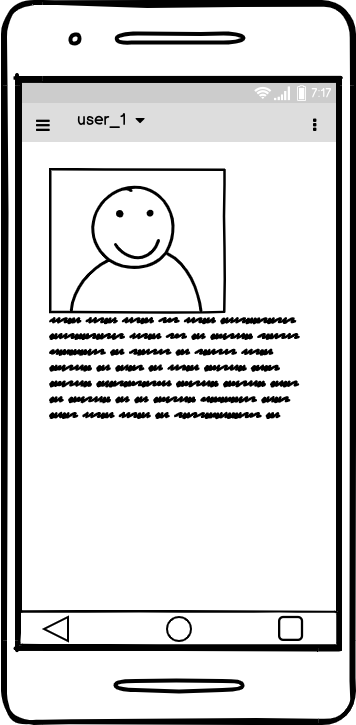
\includegraphics[width=\linewidth]{figs/user_1.png}
        \caption{User Profile} \label{fig:x_a}
    \end{subfigure}
    \hspace*{\fill}
    \begin{subfigure}{0.3\textwidth}
        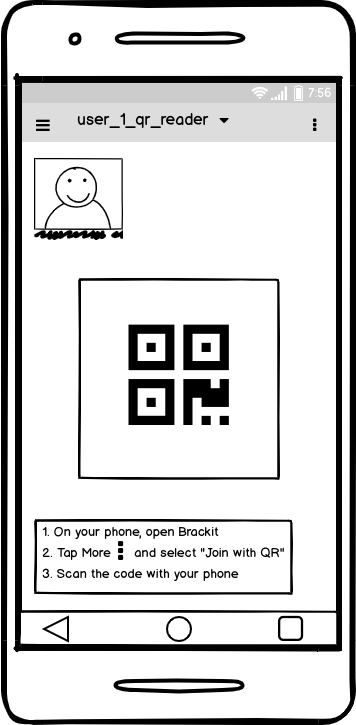
\includegraphics[width=\linewidth]{figs/user_1_qr_reader.png}
        \caption{QR Reader} \label{fig:x_b}
    \end{subfigure}
    \hspace*{\fill}
    \begin{subfigure}{0.3\textwidth}
        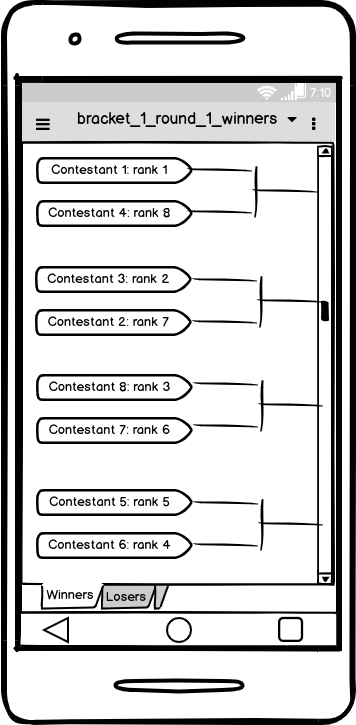
\includegraphics[width=\linewidth]{figs/bracket_1_round_1_winners.png}
        \caption{Vertical Bracket Visualization} \label{fig:x_c}
    \end{subfigure}
    \begin{subfigure}{1\textwidth}
        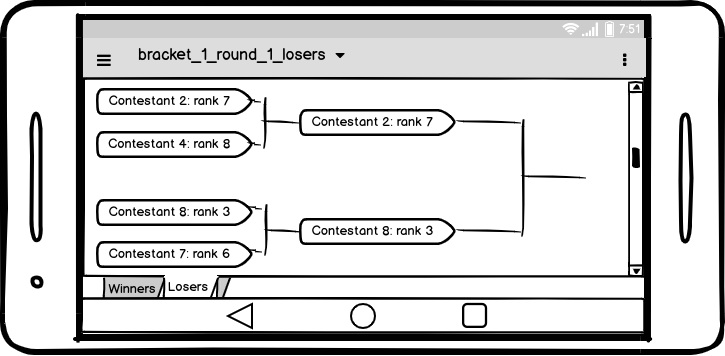
\includegraphics[width=\linewidth]{figs/bracket_1_round_2_losers.png}
        \caption{Horizontal Bracket Visualization} \label{fig:x_c}
    \end{subfigure}
\end{figure*}

\bibliography{mybib.bib}{}
\bibliographystyle{plain}
\end{document}